\documentclass[12pt]{article}
\usepackage{fancyhdr}
%\usepackage{hyperref}  -- compilation errors
\usepackage[pdftex]{graphicx}
\usepackage{amsfonts, amsmath, amssymb}
\usepackage{booktabs}
\usepackage{multirow}
\usepackage{graphicx, cite, color, setspace, url, verbatim, afterpage}
\usepackage{stfloats}
\usepackage{xspace}
\usepackage{paralist}

\usepackage{algorithm}
\usepackage[noend]{algpseudocode}
\renewcommand{\algorithmicrequire}{\textbf{Input:}}
\renewcommand{\algorithmicensure}{\textbf{Output:}}
\renewcommand{\algorithmicindent}{12pt}

\usepackage{listings}

\newcommand{\asminst}[1]{{\small\texttt{#1}}}
\newcommand{\fnm}[1]{\footnotemark[#1]}
\renewcommand{\algorithmicforall}{\textbf{for each}}

\setlength{\marginparwidth}{0.75in}
\newcommand{\MarginPar}[1]{\hspace{1sp}\marginpar{\tiny\sffamily\raggedright\hspace{1sp}{\color{red}#1}}}
\newcommand{\mc}[2]{\multicolumn{#1}{|c|}{#2}}
\newcommand{\mcf}[2]{\multicolumn{#1}{c|}{#2}}
\newcommand{\mcff}[2]{\multicolumn{#1}{c||}{#2}}
\newcommand{\mcb}[2]{\multicolumn{#1}{|c}{#2}}
\newcommand{\mcn}[2]{\multicolumn{#1}{c}{#2}}
\newcommand{\mcfd}[2]{\multicolumn{#1}{c||}{#2}}
\newcommand{\mrw}[2]{\multirow{#1}{r}{#2}}
\newcommand{\rb}[1]{\raisebox{1.5ex}[0pt]{#1}}
\newcommand{\bp}[1]{{\mbox{\boldmath $#1$}}} % for boldface numbers in table
\newcommand{\bpx}[1]{{{\color{red}\mbox{\boldmath $#1$}}}} % missing table stuff
\newcommand{\blp}[1]{#1} % maybe blue is not working
\newcommand{\fix}[1]{\textcolor{red}{\bf #1}}
\newcommand{\secref}[1]{Section~\ref{#1}}
\newcommand{\figref}[1]{Figure~\ref{#1}}
\newcommand{\HRule}{\rule{\linewidth}{0.5mm}} % Defines a new command for the horizontal lines, change thickness here

\renewcommand\labelenumi{(\theenumi)}

\newcommand{\ignore}[1]{}

\def\naive{na\"\i ve}
\def\naively{na\"\i vely}
\def\ie{{\it i.e.}}
\def\eg{{\it e.g.}}

\newcommand{\bigO}[1]{\ensuremath{\mathcal{O}\hspace{-.2em}\left({#1}\right)}}

\renewcommand{\labelitemi}{$\bullet$}

\begin{document}

\begin{titlepage}

\center % Center everything on the page

%----------------------------------------------------------------------------------------
%	HEADING SECTIONS
%----------------------------------------------------------------------------------------

\textsc{\LARGE University of California, Irvine}\\[1.5cm] % Name of your university/college
\textsc{\Large CS 216}\\[0.5cm] % Major heading such as course name
\textsc{\large Image Understanding}\\[0.5cm] % Minor heading such as course title

%----------------------------------------------------------------------------------------
%	TITLE SECTION
%----------------------------------------------------------------------------------------

\HRule \\[0.4cm]
{ \huge \bfseries Camera Mouse}\\[0.4cm] % Title of your document
\HRule \\[1.5cm]

%----------------------------------------------------------------------------------------
%	AUTHOR SECTION
%----------------------------------------------------------------------------------------

\begin{minipage}{0.4\textwidth}
	\begin{flushleft} \large
		\emph{Author:}\\
		Rohit \textsc{Zambre} % Your name
	\end{flushleft}
\end{minipage}
~
\begin{minipage}{0.4\textwidth}
	\begin{flushright} \large
		\emph{Professor:} \\
		Dr. Charless \textsc{Fowlkes} % Supervisor's Name
	\end{flushright}
\end{minipage}\\[2cm]

% If you don't want a supervisor, uncomment the two lines below and remove the section above
%\Large \emph{Author:}\\
%John \textsc{Smith}\\[3cm] % Your name

%----------------------------------------------------------------------------------------
%	DATE SECTION
%----------------------------------------------------------------------------------------

{\large \today}\\[2cm] % Date, change the \today to a set date if you want to be precise

%----------------------------------------------------------------------------------------
%	LOGO SECTION
%----------------------------------------------------------------------------------------


\includegraphics[width=0.35\textwidth]{pics/logo.jpg}

%----------------------------------------------------------------------------------------

\vfill % Fill the rest of the page with whitespace

\end{titlepage}

%=========================================================================

\section{Summary}
\label{sec:summary}

Conventionally, the mouse pointer of a computer is controlled by a peripheral device such as a mouse or a touch-pad. The goal of this project is to develop a robust computer vision system that allows its users to control a computer's mouse pointer using head movements. Such a system would undoubtedly useful for impaired users, such as those with Cerebral Palsy or those with spinal cord injuries, since they are not able to effectively use a regular mouse/touch-pad. Currently, commercial implementations of vision-based trackers to control a mouse pointer exist. Some require special accessories or hardware, such as hats or high quality cameras; some require an initial input from the user on every system-start to choose the face-patch to track~\cite{bucammouse} while some neither require any input from the user nor do they require any special hardware. In the system developed for this project, user-input is required only once and the whole head, as apposed to a fixed face-patch, is used to control the mouse pointer (similar to the iTracker by EyeTwig~\cite{eyetwig}).


\section{Technical Approach}
\label{sec:techapp}

The system consists of a camera that points towards the user. The user should be wholly within the camera's frame of view. ~\figref{fig:camview} portrays the camera's point of view. The software of the system has three primary stages and they occur in the following order: detection, tracking and control. The system flow is outlined below:

%=================================================================
\begin{figure}[htbp]
	\begin{center}
		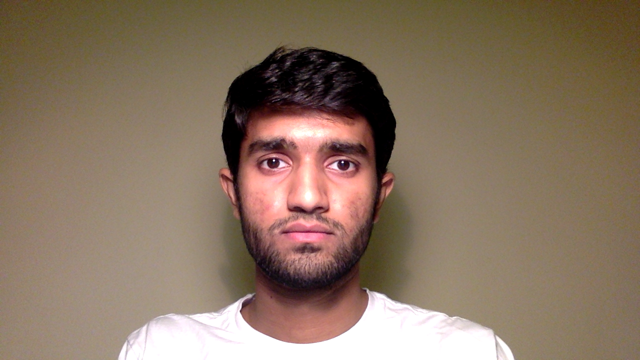
\includegraphics[width=\textwidth]{pics/cameraView.png}
	\end{center}%
	\caption{Camera's Frame of View}
	\label{fig:camview}
\end{figure}%
%=================================================================

\begin{enumerate}
	\item The user first selects their face by drawing a rectangular box around it. The selected face is used as template whenever the face needs to be detected.
	\item Once the face is detected, the system extracts features from the detected region.
	\item The extracted features are then tracked as the user moves their head around in order to control the mouse pointer.
	\item The movement of the user's head is translated into movement of the mouse pointer on the computer.
	\item If the tracked features are lost at any point during the tracking phase, the face is detected again using the template that was provided by the user in (1).
\end{enumerate}

The following subsections describe the ways in detection, tracking and pointer-control are performed. 

\subsection{Face Detection}

The system performs detection using template matching of Histogram Of Gradients (HOG). To perform detection, the HOG of the user's face (initially selected by the user) is matched against the HOG of the image that corresponds to the camera's view. The HOGs of an image is computed by dividing the image into $8\times8$ disjoint block of pixels. The orientation of each of these blocks is binned into 9 equal spaced bins between $-pi/2$ and $pi/2$. Hence, an image with height, $H$, and width, $W$, will have a HOG represented by a three-dimensional array with the dimensions of $H/8 \times W/8 \times 9$. Cross-correlation is used to compare the HOGs of two images. After performing non-maxima suppression, the $8 \times 8$ block with the largest cross-correlation measure is considered to be the center of the detected face. ~\figref{fig:detection} depicts the HOG of the face region selected by the user and the resulting detection on the camera's frame of view.

%=================================================================
\begin{figure}[htbp]
	\centering
	%-------------------------------------------------------------------------------------------
	\begin{minipage}[t]{0.24\textwidth}\centering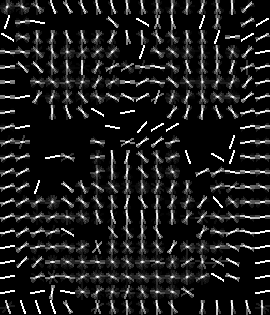
\includegraphics[width=\textwidth]{pics/faceHOG.png}\par(a) Face's HOG \end{minipage}
	\begin{minipage}[t]{0.74\textwidth}\centering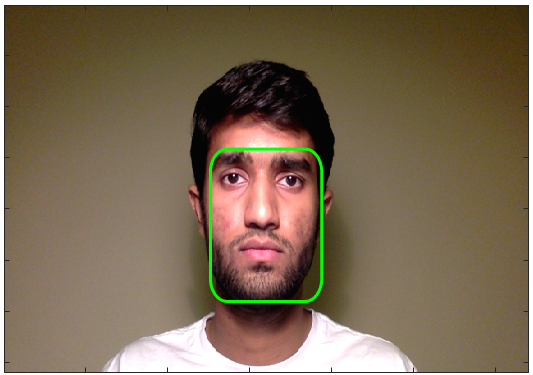
\includegraphics[width=\textwidth]{pics/detectedFace.png}\par(b) Detected Face \end{minipage}
	%-------------------------------------------------------------------------------------------
	\caption{Face detection using HOG}
	\label{fig:detection}
\end{figure}
%=================================================================

\subsection{Face Tracking}

Once the face is detected, the initial features in the detected region are extracted using the minimum eigenvalue algorithm ~\cite{shi1994good} (see Section ~\ref{sec:discussion} for initial approaches used).~\figref{fig:features} depicts the features selected by this algorithm.

The feature points are then tracked using the Kanade-Lucas-Tomasi (KLT) algorithm ~\cite{tomasi1991detection}. In order to make the tracking robust, the threshold for the bidirectional error of the KLT is set to 3 pixels. To implement the feature extraction and the tracking algorithms, I used the MATLAB functions and objects, \texttt{detectMinEigenFeatures}~\cite{mineigen} and \texttt{PointTracker}~\cite{pointtracker} from the Computer Vision System Toolbox ~\cite{cvtoolbox}. If the lighting conditions are not constant or if the head movements are too fast, a significant portion of the feature trackers are lost. Hence, when less than 10 feature points remain, the system notifies the user about the loss of tracking, asks the user to stay still and re-detects the face of the user using the HOG of the template specified by the user. ~\figref{fig:tracking} shows the tracking of the same features in different head poses. The red star in the figure demarcates the head-position (the mean position of all features)

%=================================================================
\begin{figure}[htbp]
	\begin{center}
		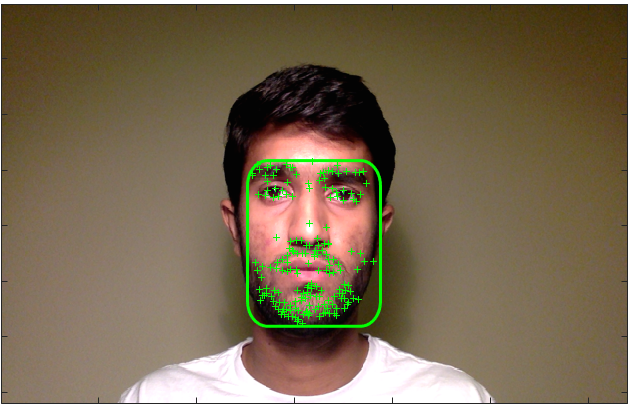
\includegraphics[width=0.9\textwidth]{pics/detectedFeatures.png}
	\end{center}%
	\caption{Features detected by the minimum eigenvalue algorithm}
	\label{fig:features}
\end{figure}%
%=================================================================


%=================================================================
\begin{figure*}[htbp]
	%\vspace{-20pt}
	\centering
	%-----------------------------------------------------------------------------------------
	\begin{minipage}[t]{0.49\textwidth}\centering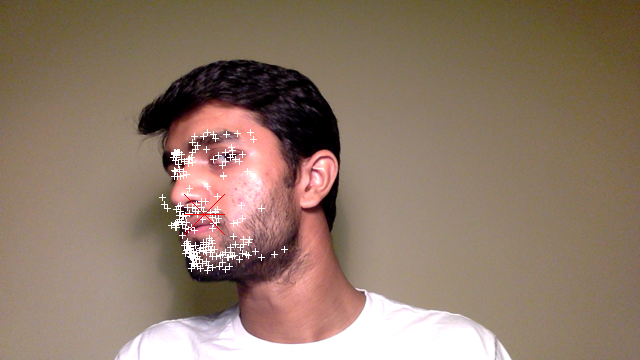
\includegraphics[width=\textwidth]{pics/leftTracking.png}\par(a) Facing Left  \end{minipage}
	\begin{minipage}[t]{0.49\textwidth}\centering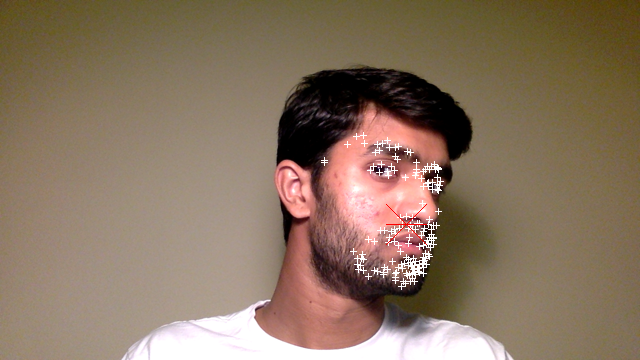
\includegraphics[width=\textwidth]{pics/rightTracking.png}\par(b) Facing Right \end{minipage}
	\begin{minipage}[t]{0.49\textwidth}\centering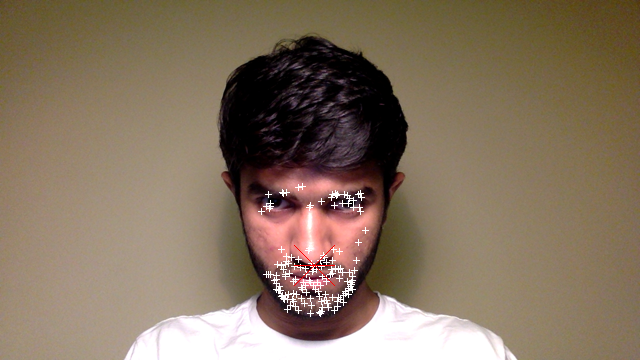
\includegraphics[width=\linewidth]{pics/downTracking.png}\par(c) Facing Down \end{minipage}
	\begin{minipage}[t]{0.49\textwidth}\centering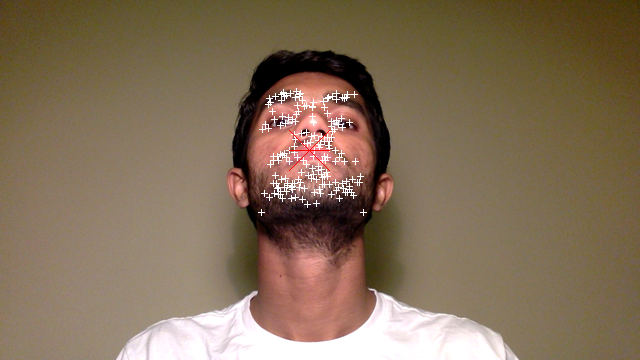
\includegraphics[width=\linewidth]{pics/upTracking.png}\par(d)  Facing Up \end{minipage}
	%-----------------------------------------------------------------------------------------
	\caption{Feature tracking in different head poses.}
	\label{fig:tracking}
\end{figure*}
%=================================================================



\subsection{Pointer Control}

To control the mouse pointer according to the head movements, I use a linear Rate Control approach ~\cite{kjeldsen2006improvements}. In a Rate Control approach, the movement of the pointer depends only on the succeeding motions of the head and doesn't consider any absolute reference position/frame.

When the face has been detected and the tracker has been initialized, I se the mouse pointer to the center of the screen. In every frame, I compute the mean of the x-coordinates of all the feature points and the mean of the y-coordinates of all the feature points being tracked and use the resulting means to demarcate the "head-position." I compute the displacement, $x$ of this position w.r.t the same in the previous frame. I apply $Ax$, a scaled version of this displacement to determine the next coordinates of the mouse pointer. Empirically, a value of 15 for $A$ worked reasonably well.
\section{Results}
\label{sec:results}

Under constant lighting conditions and steady head movements, the system performs fairly well; more than 10 tracking features are successfully tracked for 500 frames. With regular tracking and display of the tracking features, the systems achieves a frame rate of $9.08$ fps. Without the display of the tracking features, the system achieves a frame rate of $10.25$ fps. With no feedback at all, the system achieves a frame rate of $18.88$ fps.

To further evaluate the performance of the tracking, we compared the head position determined by the system to the head position manually marked by the user. Over a set of $500$ frames, I compared the user's true head position and that determined by the system for every $100th$ frame. On an average, the Euclidean distance between the true head-position and the mean head-position was $401$ pixels which is $1.06\%$ of the face template's diagonal length.

A demonstration of the system's current implementation is available on YouTube~\cite{demo}.


\section{Discussion}
\label{sec:discussion}

\textbf{Feature-tracking} Before implementing minimum eigenvalue feature-extraction method, I had initialized the KLT tracker on a central portion of the detected face region by removing a length of 25 pixels from each side of the box. Hence, if the detected face region had a size of $H \times W$, the resulting size of the central patch was $(H-50) \times (W-50)$. All the pixels in this central region served as "feature-trackers" for the box. Although the tracking with such an approach was very robust, the performance was quite slow since the number of features to track were very large.

\textbf{Limitations} The system implemented in this project carries limitations that generally come with a simple computer vision system.
\begin{itemize}
	\item Under \textbf{non-uniform lighting}, the majority of the features selected by the minimum eigenvalue algorithm are on the brighter side of the face. Hence, when the user moves their head sideways, a majority of the features are lost. 
	\item The KLT tracker cannot handle \textbf{rapid head movements} of the head. Any rapid head movement or even a quick drastic change in the expression of the user's face can cause the loss of all tracking points.
	\item Using the mean position of the feature-trackers to determine the head-position sometimes causes the mouse-pointer to "drift." This occurs when some of the tracking-features are lost during the head movements causing a small change in the mean position of the features.
\end{itemize}

\textbf{Future work.} Overall, the current implementation performs fairly well under uniform lighting and with regular, steady head movements. However, the current technical approaches cannot be deployed to a commercial implementation of such a system. Some ways in which the system can be improved:
\begin{itemize}
	\item \textbf{Improved feature selection}. Once the region of the face has been detected, instead of finding the corners using the minimum eigenvalue algorithm, the system could use a face landmark estimation algorithm that captures the key features on the face. Burgos-Artizzu et al. ~\cite{burgos2013robust} demonstrate a robust algorithm that does exactly this even under occlusion.
	\item \textbf{Improved tracking}. The system could definitely use a more robust tracking algorithm for the purpose of tracking simple and steady head movements. Epstein et al. ~\cite{epstein2014using} propose the use of kernel-projections for their implementation of a camera mouse in which they track a user-specified patch on the face.
\end{itemize}




%=========================================================================
\bibliographystyle{abbrv}
\small
\bibliography{main}
%=========================================================================
\normalsize
%\input{appendix}
%=========================================================================
\end{document}
